\chapter{Rešerše}
\label{2-reserse}

Tato kapitola shrnuje základní informace o~systému \zkratka{DORIS} a službě \zkratka{IDS}. Dále jsou představeny existující práce zabývající se analýzou časových řad souřadnic stanic a porovnáváním přesných drah družic. V~dostupné literatuře nebyla nalezena komplexní práce, která by se zabývala současně analýzou časových řad souřadnic stanic systému \zkratka{DORIS} a porovnáním přesných drah družic z~různých analytických center \zkratka{IDS}. Existuje však řada prací, které se těmito oblastmi zabývají samostatně nebo v~širším kontextu.

\section{Základní informace o~systému DORIS}

Systém \zkratka{DORIS} je založen na využití Dopplerova jevu, k~němuž dochází v~důsledku relativního pohybu mezi pozemní vysílací stanicí a družicí vybavenou přijímačem. Pozemní stanice vysílají signál o~známé frekvenci, přičemž palubní přijímač na družici měří jeho frekvenční posun. Tento posun je přímo závislý na relativní rychlosti družice vůči stanici a představuje základní observaci využívanou při přesném určování drah družic. Systém \zkratka{DORIS} poskytuje dva typy observací, a to dopplerovská a synchronizační měření. Na palubě družice je měření realizováno sledováním fáze přijímaného signálu, přičemž změna fáze v~čase odpovídá změně frekvence, z~níž je následně odvozena Dopplerovská observace využívaná při zpracování dat. Synchronizační měření slouží především pro časovou vazbu mezi palubními a pozemními časovými škálami~\cite{ids_what_is_doris}.

\subsection{Princip měření}

Na rozdíl od globálních navigačních satelitních systémů \zk{GNSS}, kde jsou vysílače umístěny na družicích a přijímače na zemském povrchu, využívá systém \zkratka{DORIS} opačné uspořádání. Vysílače se nacházejí na pozemních stanicích, zatímco přijímače jsou umístěny na družicích. Díky tomu je technicky náročnější část systému umístěna na Zemi a na družicích se nachází konstrukčně jednodušší část systému~\cite{ids_what_is_doris}.

Pozemní stanice \zkratka{DORIS} vysílají nepřetržitý signál současně na~dvou frekvencích (2036,25~MHz a~401,25~MHz), jejichž kombinace umožňuje potlačení vlivu ionosféry~\cite{ids_frequency_shift}. Stabilita těchto vysílaných frekvencí je stěžejní pro~přesnost měření, jelikož jakákoliv nestabilita by se přímo promítla do~odhadu relativní rychlosti~\cite{ids_what_is_doris}. U~vybraných stanic se navíc využívá mírný posun frekvence oproti nominální hodnotě. To se aplikuje v~situacích, kdy se dvě stanice nacházejí v~blízké geografické poloze, čímž se předchází vzájemnému rušení signálů~\cite{ids_frequency_shift}.

Palubní přijímač na družici měří fázi přijímaného signálu, ze~které se odvozuje frekvenční posun způsobený relativním pohybem mezi družicí a stanicí. Pozemní stanice vysílá signál o~známé frekvenci \(f_0\), zatímco frekvence signálu přijímaného na družici je označena \(f_r\). Rozdíl mezi těmito frekvencemi odpovídá Dopplerovu posunu, který přímo souvisí s~relativní rychlostí družice vůči stanici. Při přibližování družice ke stanici platí \(f_r > f_0\), při vzdalování \(f_r < f_0\). Měřením časového průběhu této změny během průletu družice nad~stanicí se získává základní observace využitelná při~přesném určení dráhy družice. Schéma tohoto principu je znázorněno na obr.~\ref{fig:doris_system}.

\begin{figure}[H]
    \centering
    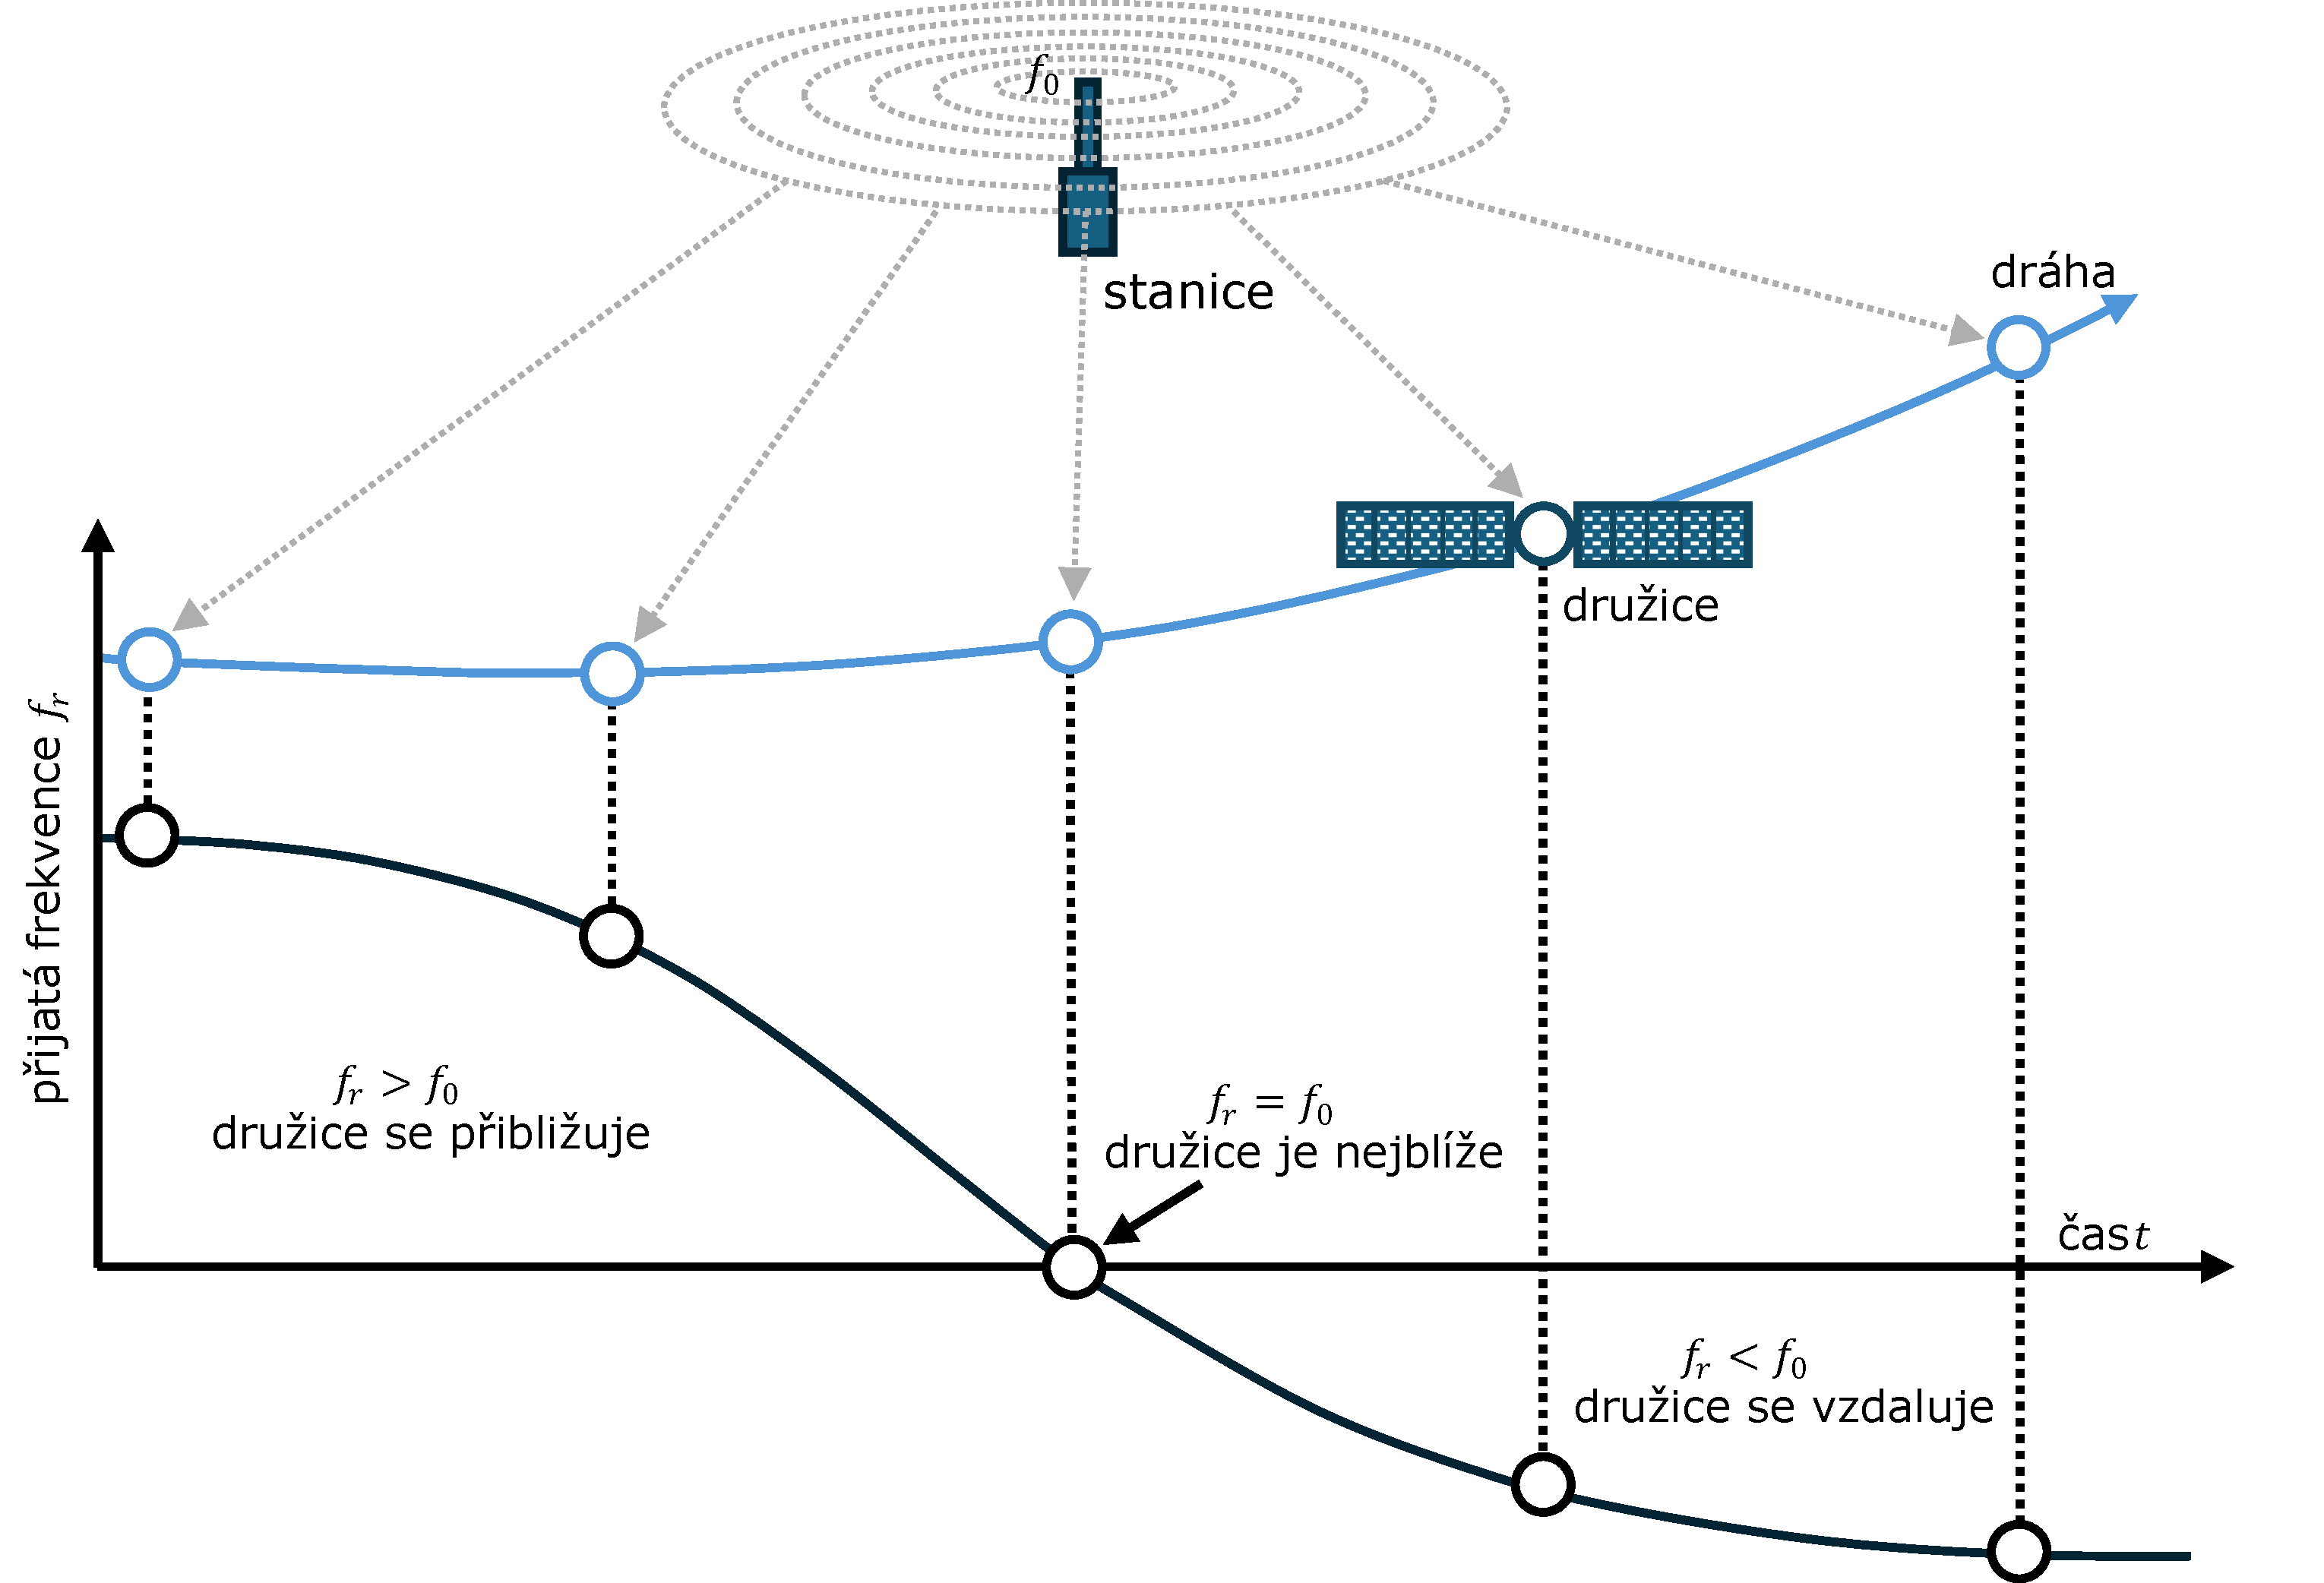
\includegraphics[width=1\linewidth]{images/Doris_doppler.pdf}
    \caption{Schéma principu měření systému DORIS (podle~\cite{ggos_doris})}
    \label{fig:doris_system}
\end{figure}

Výhodou uspořádání systému \zkratka{DORIS} je relativní konstrukční jednoduchost palubního přijímače, jeho nižší energetická náročnost a menší prostorové požadavky. Díky tomu může být systém \zkratka{DORIS} integrován i na družice, jejichž primární mise není geodetická, ale například altimetrická, oceánografická, zaměřená na studium kryosféry nebo na dálkový průzkum Země.

\subsection{Struktura IDS}

\zkratka{IDS} je mezinárodní služba působící v~rámci organizací \zkratka{IAG} a \zkratka{GGOS}. Jejím hlavním cílem je koordinace zpracování dat systému \zkratka{DORIS} a publikace oficiálních produktů. \zkratka{IDS} se skládá z~několika složek (viz obr.~\ref{fig:ids_structure})~\cite{ggos_ids}. Nejvyšším orgánem je Governing Board, který určuje strategii rozvoje služby, schvaluje standardy a koordinuje spolupráci s~ostatními geodetickými službami. Organizační a komunikační činnost zajišťuje Central Bureau, které spravuje dokumentaci, technické standardy a organizuje odborná setkání. Datová centra (Data Centers) slouží k~archivaci a distribuci surových i zpracovaných dat, včetně měření ve formátu \texttt{RINEX}, řešení analytických center a kombinovaných produktů. Analytická centra (Analysis Centers) nezávisle zpracovávají data systému \zkratka{DORIS} a poskytují řešení drah družic, souřadnic stanic a parametrů orientace Země. Mezi významná analytická centra patří například CNES/\allowbreak CLS, IGN, NASA/\allowbreak GSFC nebo ESOC, přičemž důležitým přispěvatelem je také Geodetická observatoř Pecný (\zk{GOP}). Výsledná nezávislá řešení jednotlivých analytických center jsou následně slučována do jednoho oficiálního řešení \zkratka{IDS} v~rámci kombinačního centra (Combination Center), které vytváří oficiální produkty \zkratka{IDS}~\cite{ids_structure}.

\begin{figure}[H]
    \centering
    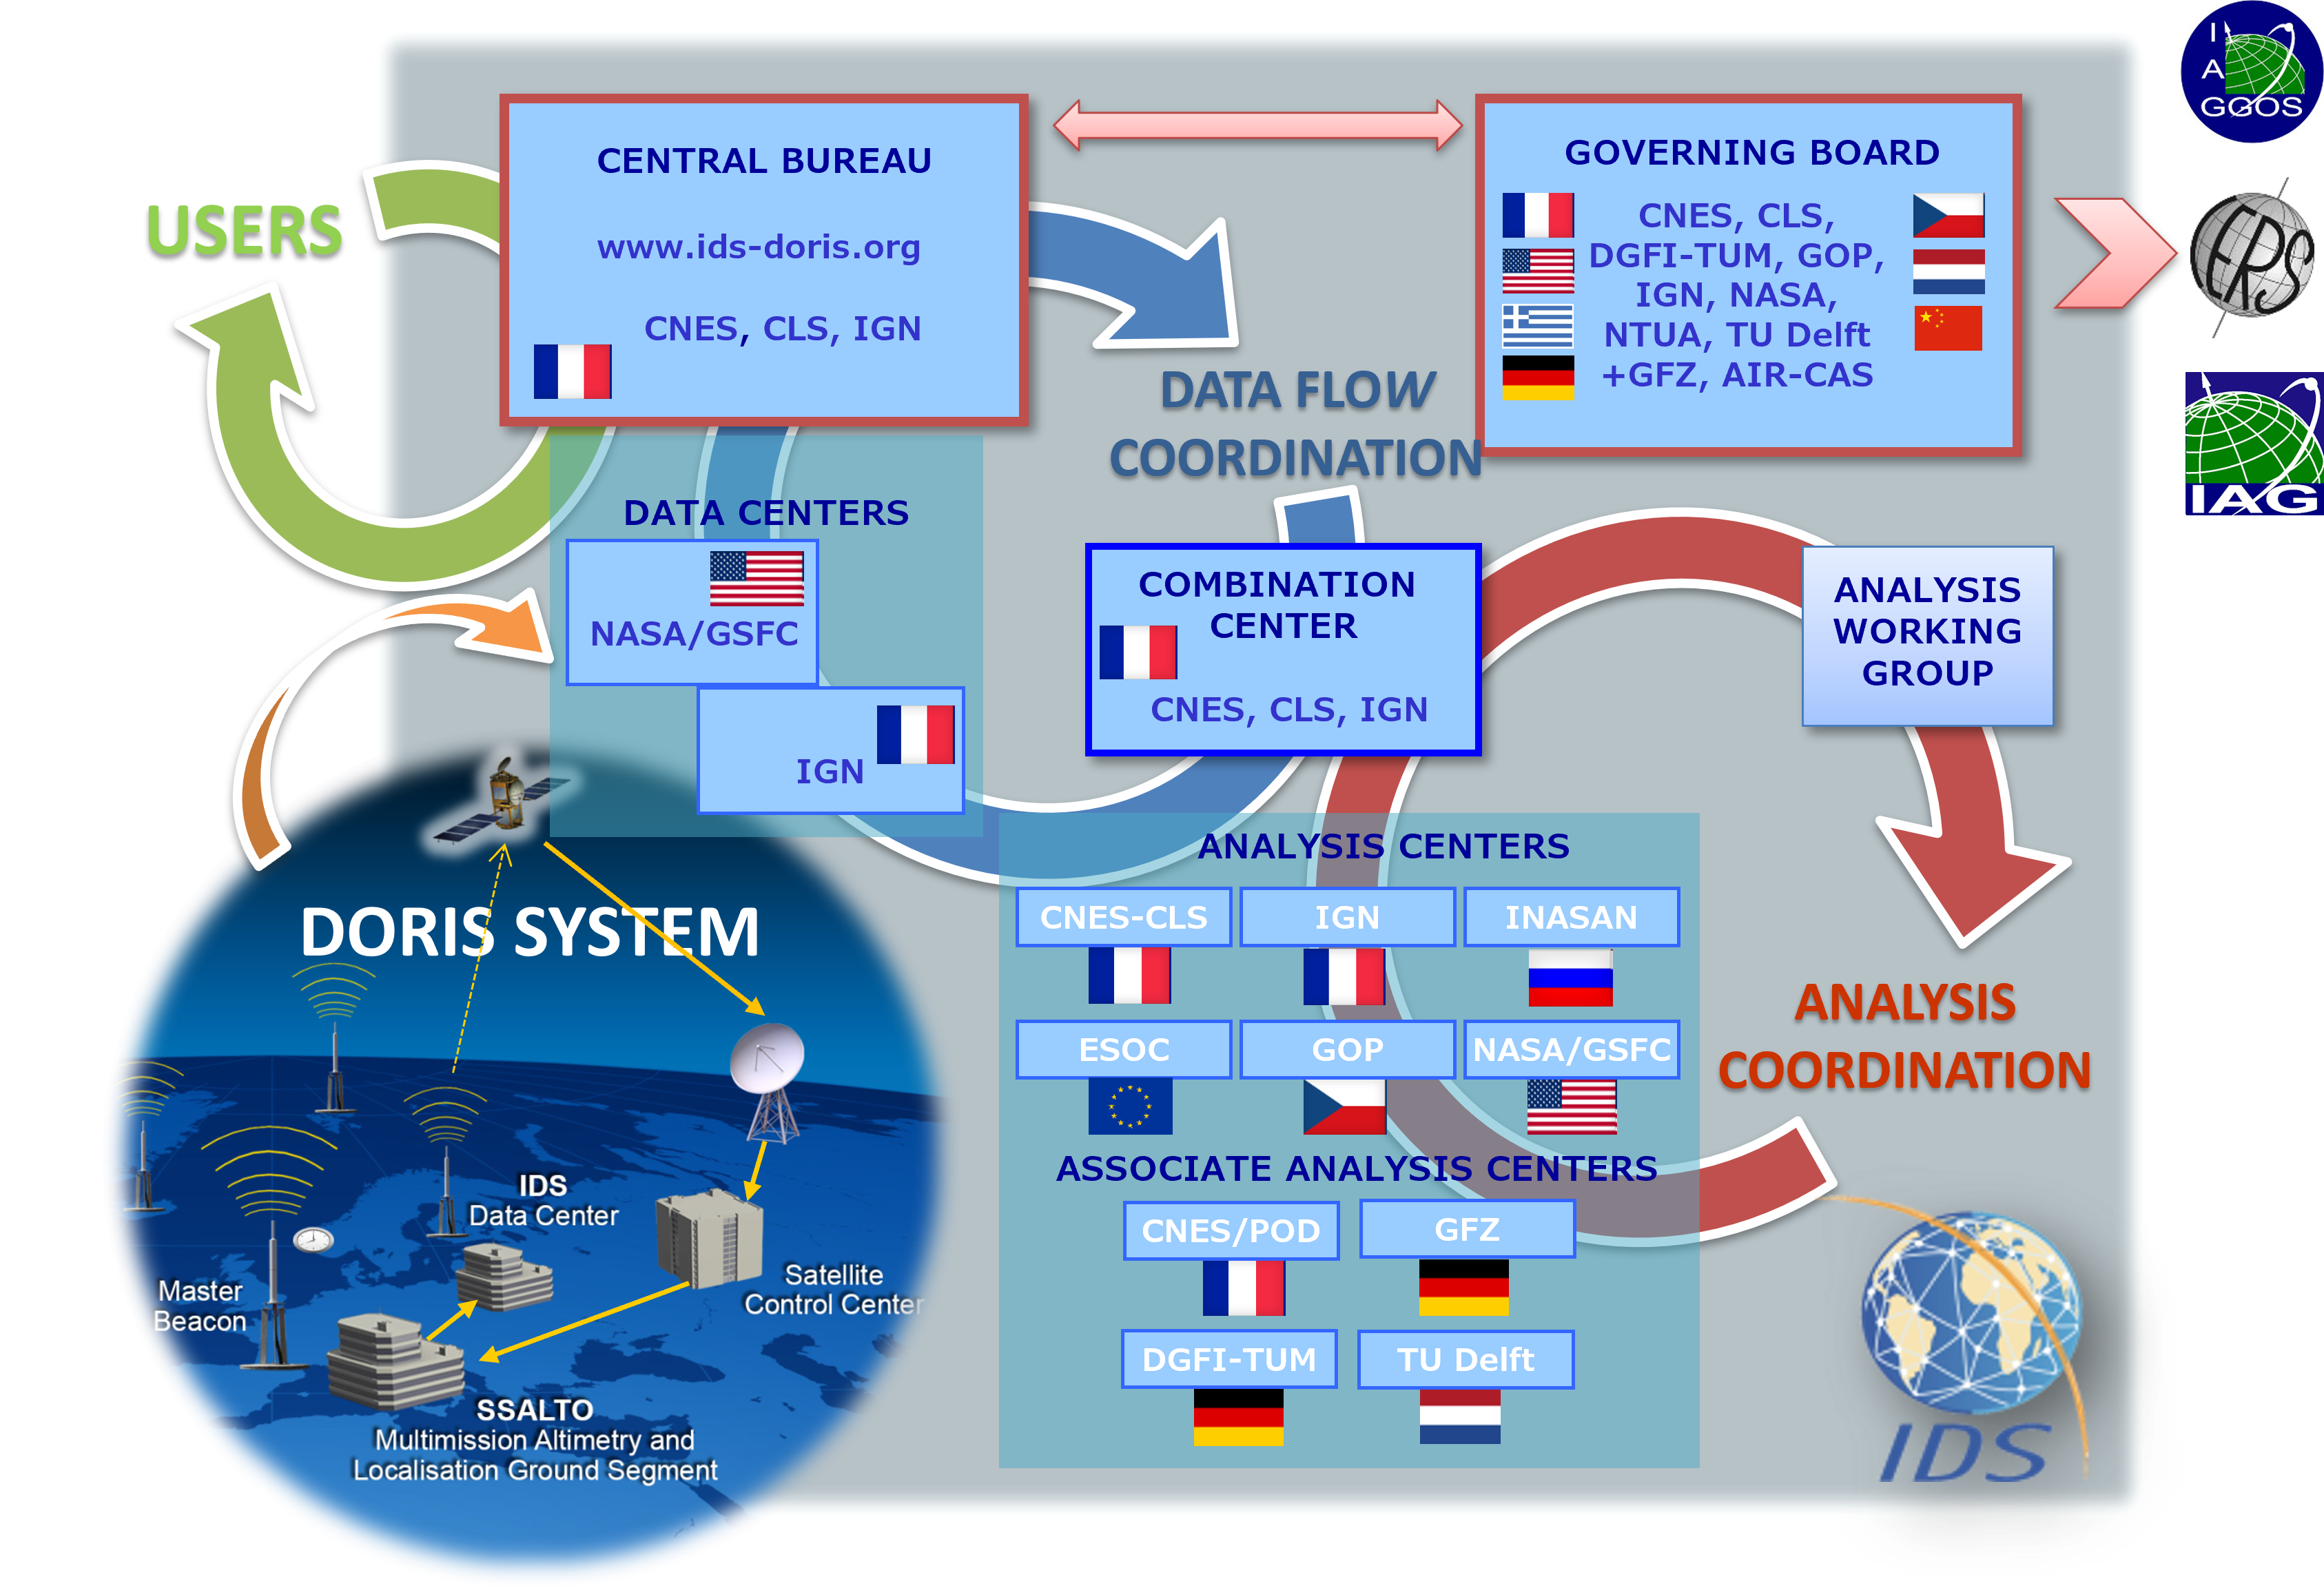
\includegraphics[width=0.9\linewidth]{images/Struktura_ids.png}
    \caption{Struktura služby IDS (převzato z~\cite{ids_structure})}
    \label{fig:ids_structure}
\end{figure}

\subsection{Přínos systému DORIS}

Produkty služby \zkratka{IDS} jsou využívány k~mnoha aplikacím v~oblasti geodézie a \mbox{geodynamiky}. Systém \zkratka{DORIS} slouží především pro přesné určování drah družic, které jsou nezbytné například pro altimetrické mise a dálkový průzkum Země. Kromě toho umožňuje určování souřadnic a rychlostí pozemních stanic, stanovení parametrů orientace Země a sledování změn polohy geocentra~\cite{moreaux_2023_itrf2020}. Díky dlouhodobým časovým řadám souřadnic stanic lze data systému \zkratka{DORIS} využít také pro studium geodynamických procesů, jako jsou pohyby tektonických desek nebo deformace zemské kůry. Systém \zkratka{DORIS} patří vedle dalších technik kosmické geodézie, jako jsou \zkratka{GNSS}, \zkratka{SLR} a \zkratka{VLBI}, mezi klíčové zdroje dat využívané při realizaci \mbox{mezinárodního} terestrického referenčního rámce (\zk{ITRF}). Přínos služby \zkratka{IDS} k~realizaci \zk{ITRF}2020 je podrobně popsán například v~práci Moreaux et al.~\cite{moreaux_2023_itrf2020}, která hodnotí kvalitu a stabilitu řešení poskytovaných jednotlivými analytickými centry. Na úrovni konkrétních řešení se problematikou zpracování dat systému \zkratka{DORIS} zabývají také Štěpánek et al.~\cite{stepanek_2023_gop_itrf2020,stepanek_2006_doris_data_analysis}, kteří popisují přístup Geodetické observatoře Pecný a její příspěvek k~mezinárodním kombinacím. Dále Schreiner et al.~\cite{schreiner_2023_pod_doris_gps_slr} ukazují, že kombinace technik \zkratka{DORIS}, \zkratka{GPS} a~\zkratka{SLR} vede ke~zvýšení přesnosti drah u~misí Sentinel-3 a~Sentinel-6.

\section{Základní informace o~časových řadách}

Analýza časových řad souřadnic geodetických stanic je standardně využívána pro hodnocení stability geodetických sítí a kvality zpracování dat. Z~toho důvodu je problematika časových řad souřadnic stanic v~literatuře podrobně zpracována. V~případě stanic systému \zkratka{DORIS} mají tyto analýzy význam také pro hodnocení konzistence řešení poskytovaných jednotlivými analytickými centry \zkratka{IDS}, jejichž kombinací vzniká oficiální řešení~\cite{moreaux_2023_itrf2020}. Časové řady jsou obvykle modelovány jako kombinace trendu, periodických složek a případných diskontinuit, které mohou vznikat například v~důsledku změn ve zpracování, v~měření nebo geofyzikálních jevů. Přehled metod analýzy těchto časových řad poskytují například Bos et al.~\cite{bos_2019_time_series}, kteří popisují tzv. trajectory model zahrnující uvedené složky.

Dlouhodobý trend časové řady je nejčastěji odhadován metodou nejmenších čtverců, jejíž teoretické základy jsou detailně vysvětleny například v~publikaci \mbox{Montgomery} et al.~\cite{montgomery_regression}. V~praxi je přitom nutné zvolit vhodný model trendu. Z~tohoto důvodu je vhodné uvažovat více kandidátních modelů, přičemž pro jejich porovnání lze využít různá informační kritéria, například Bayesovské informační kritérium (\zk{BIC}), které umožňuje zohlednit jak kvalitu aproximace, tak složitost modelu~\cite{kass_raftery_1995}.

Pro analýzu periodických složek časových řad se využívá spektrální analýza. Mezi nejběžnější metody spektrální analýzy patří zejména rychlá Fourierova trans\-formace (\zk{FFT})~\cite{cooley_tukey_1965} a Lomb--Scargleův periodogram, který je vhodný pro nepravidelně vzorkovaná data~\cite{lomb_scargle}.

Detekce zlomů umožňuje identifikovat změny statistických vlastností časových řad. Přehled metod pro detekci zlomů uvádí například Truong et al.~\cite{change_point_review}.

Popis šumu, tedy náhodné složky dat, je rozebrán v~práci Bos et al.~\cite{bos_2019_time_series}. Šum v~časových řadách obvykle není čistě bílý, ale vykazuje časovou závislost, a proto je často modelován jako kombinace více typů šumu.

\section{Základní informace o~drahách družic}

Přesné určování drah družic je jednou z~klíčových úloh v~oblasti kosmické geodézie a dálkového průzkumu Země. Přesnost určení dráhy má zásadní vliv na kvalitu výsledků altimetrických měření, navigačních aplikací i geodetických produktů.

Pro dosažení vyšší přesnosti bývají využívány kombinace různých technik kosmické geodézie, mezi které patří například \zkratka{DORIS}, \zkratka{GPS} a \zkratka{SLR}. Problematikou přesného určování drah družic pomocí kombinace těchto technik se zabývají například Schreiner et al.~\cite{schreiner_2023_pod_doris_gps_slr}, kteří analyzují řešení drah družic Sentinel-3A/B a Sentinel-6A. Kombinací metod \zkratka{SLR} a \zkratka{DORIS} se zabývá také práce Zeitlhöfler et al.~\cite{zeitlhoefler_2025_combined_orbit_slr_doris}.

Pro zhodnocení konzistence jednotlivých řešení drah družic se provádí jejich vzájemné porovnání na základě rozdílů polohy družice mezi jednotlivými řešeními. Rozdíly drah družic jsou vyjadřovány buď v~kartézském souřadnicovém systému, nebo v~lokálním orbitálním referenčním systému \zkratka{RTN}, který umožňuje fyzikální interpretaci odchylek~\cite{schreiner_2023_pod_doris_gps_slr}. Pro kvantitativní hodnocení se využívají statistické charakteristiky, zejména kvadratická odchylka (RMS)~\cite{stepanek_2023_gop_itrf2020}.

Vzhledem k~tomu, že data nejsou vždy poskytována ve stejné časové škále a nejsou vzorkována ve stejných epochách, je nutné je převést na jednotnou časovou osu a případně interpolovat na společné epochy. Konkrétní interpolační metody jsou podrobně rozebrány v~\cite{zeitlhoefler_2024_interpolation}, kde jsou porovnávány různé přístupy. Jedním z~nich je Hermitova interpolace, která je výhodná, jelikož kromě polohy využívá i rychlost družice, tedy první derivaci dráhy.

\section{Shrnutí současného stavu}

Z~rešerše vyplývá, že jednotlivá témata jako systém \zk{DORIS}, dráhy družic a analýza časových řad jsou dobře popsána. Nebyla však nalezena práce, která by se komplexně zabývala současně analýzou časových řad souřadnic stanic systému \zk{DORIS} a zároveň porovnáním přesných drah družic z~různých analytických center \zkratka{IDS}. Přesto lze z~existujících metod a postupů vycházet a vhodně je kombinovat pro účely této práce.